\documentclass[11pt,letterpaper]{article}

\usepackage[margin=1in]{geometry}
\usepackage{graphicx}
\usepackage{booktabs}
\usepackage{amsmath}
\usepackage{siunitx}
\usepackage{float}
\usepackage{hyperref}
\usepackage[nameinlink,noabbrev]{cleveref}
\usepackage{microtype}

\graphicspath{{figures/}}
\sisetup{per-mode=symbol}
\hypersetup{colorlinks=true, linkcolor=blue, citecolor=blue, urlcolor=blue}

\title{Comparing Matrix Multiplication Implementations Across CPU and GPU Platforms}
\author{\textbf{YOUR NAME}\\[0.4em]
        \small YOUR COURSE / INSTITUTION}
\date{\today}

\begin{document}
\maketitle

\begin{abstract}
% TODO (150--250 words): State the question, implementations, machine, principal
% measurements, main result, and the most important limitation. Avoid claiming
% that the implementations are equivalent in precision or timing scope unless
% you verify that they are.
\end{abstract}

\section{Introduction}
% TODO: Motivate matrix multiplication as a useful kernel for comparing
% implementation strategies. State the research question and summarize what
% the reader should learn from the comparison.

\section{Implementations}
% TODO: Describe the seven implementations and point readers to their source:
% pure Python loops; NumPy; PyTorch CPU/GPU; naive and blocked Triton; naive and
% tiled CUDA C++. Explain how each GPU kernel maps output work to programs,
% blocks, or threads, and what data reuse its tiling provides.

\section{Experimental Method}
\subsection{Hardware and software}
% TODO: Record GPU model and memory, CPU model and core count, operating system,
% Python, CUDA toolkit/driver, PyTorch, Triton, NumPy versions, and relevant
% environment settings. Explain whether other GPU work was running.

\subsection{Workload and correctness}
% TODO: State matrix dimensions, dtypes, input generation, and number of runs.
% Describe how outputs were checked against a trusted reference, including the
% tolerance used. If you did not validate correctness, say so clearly.

\subsection{Timing procedure}
% TODO: Explain that CPU calls use host wall-clock timing and GPU samples use
% CUDA graph timing aggregates. Inputs and output buffers are prepared outside
% the GPU sample timing. Warm-up is recorded separately; CUDA extension loading
% occurs before its timed warm-up, while Triton compilation can occur during its
% first call. These measurements therefore have different timing scopes.
%
% State the sample count: the current saved run has 30 measured samples for
% each implementation except pure Python, which has one. The CSV files are in
% ../Data/benchmark_results.csv and ../Data/benchmark_raw_logs.csv.

\subsection{Precision}
% TODO: Document the precision modes used by PyTorch, Triton, and CUDA. In
% particular, state whether Triton's tl.dot used TF32 or IEEE FP32 and whether
% PyTorch matmul precision was explicitly configured. Do not describe this as
% an equal-precision comparison unless the settings were matched.

\section{Results}
% TODO: Lead with the central observations. Quote mean and median timings in
% milliseconds, identify sample counts, and describe variability. Distinguish
% observed timing differences from explanations of those differences.

\begin{figure}[p]
  \centering
  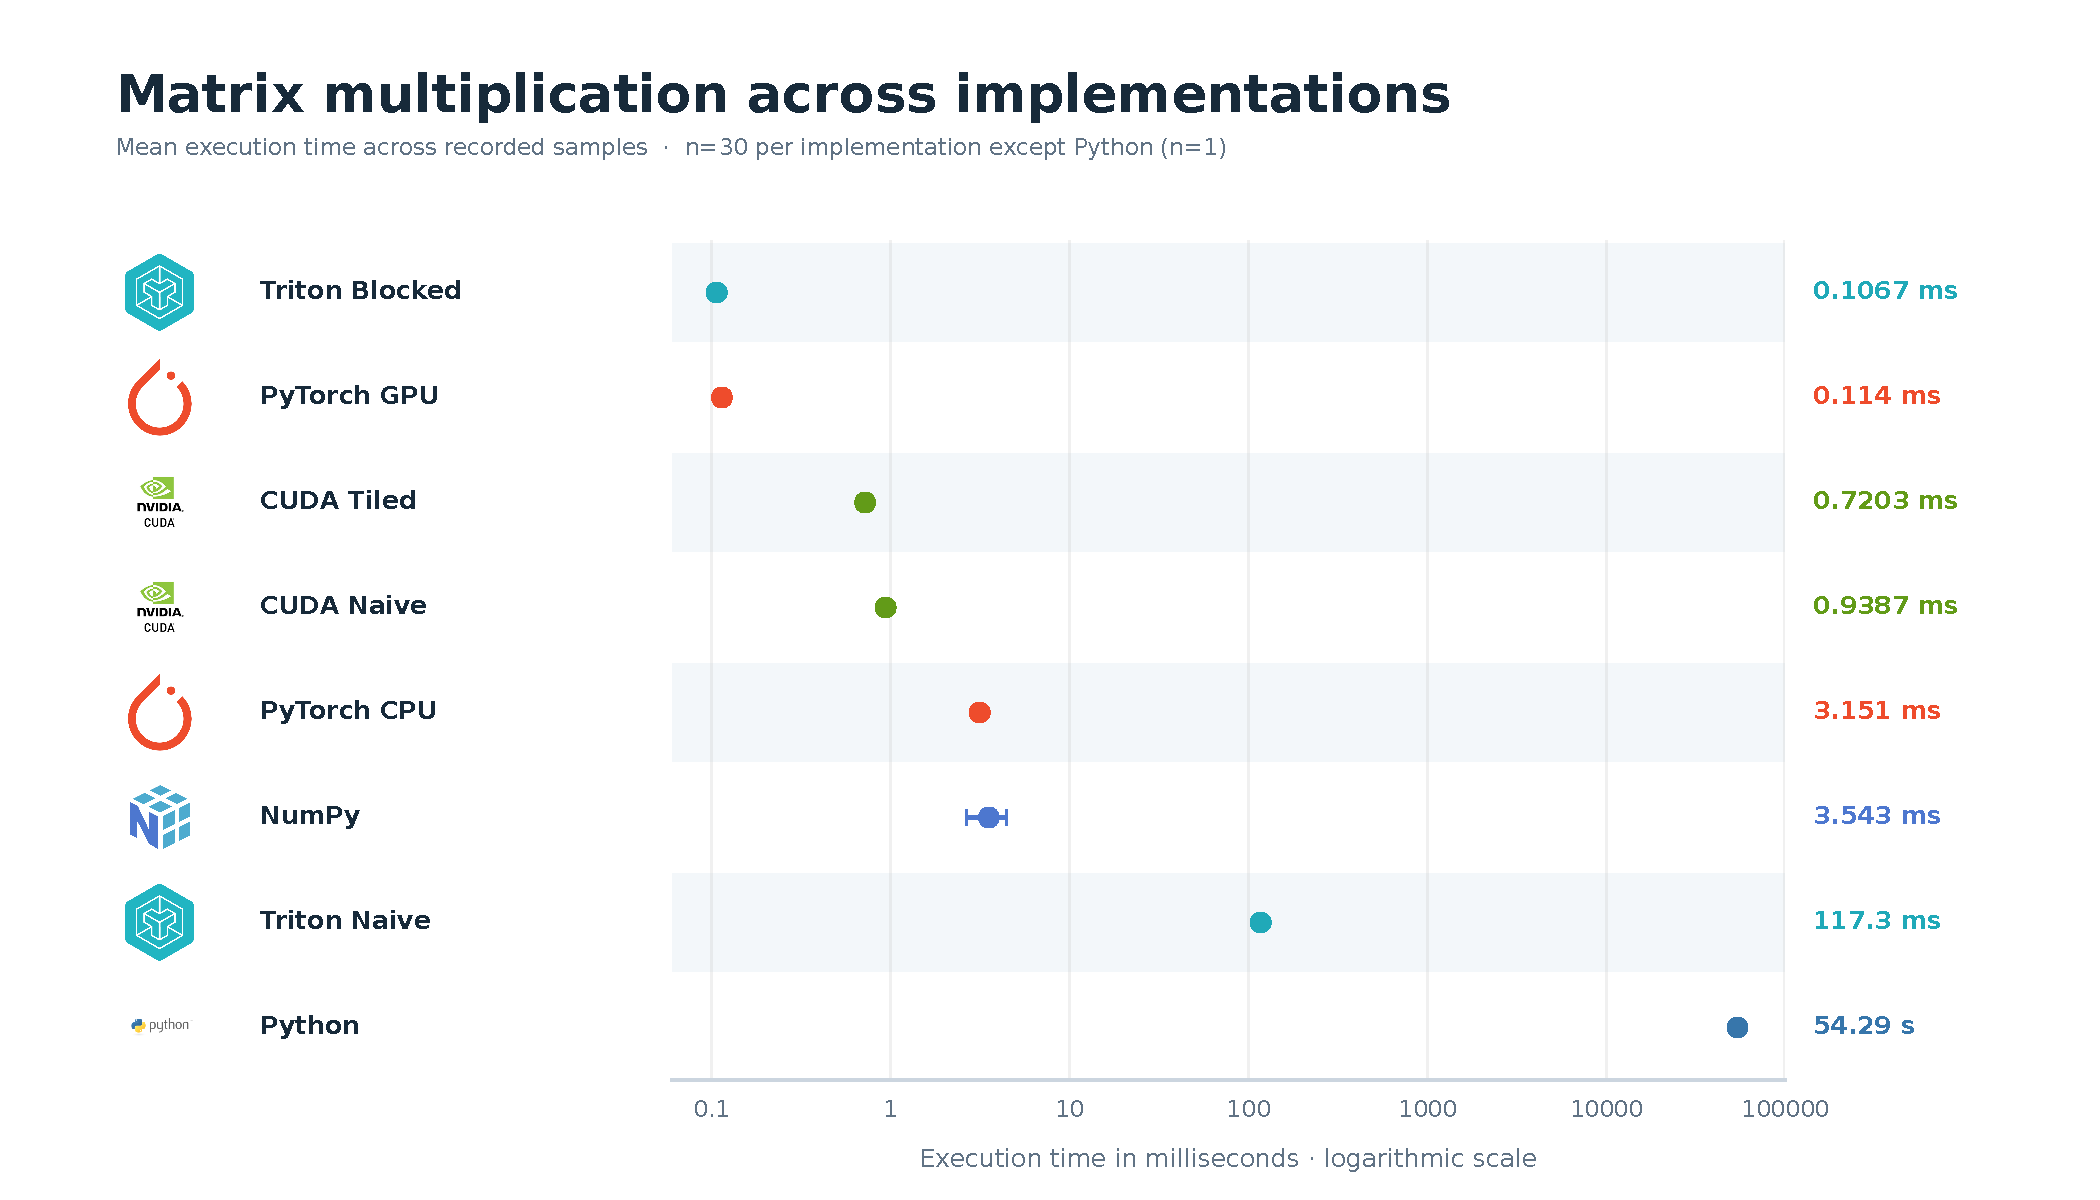
\includegraphics[width=0.98\textwidth,height=0.82\textheight,keepaspectratio]{01_overview.pdf}
  \caption{Mean execution time across implementations. The horizontal axis is logarithmic. Python has one measured sample; other implementations have 30.}
  \label{fig:overview}
\end{figure}
\clearpage

\begin{figure}[p]
  \centering
  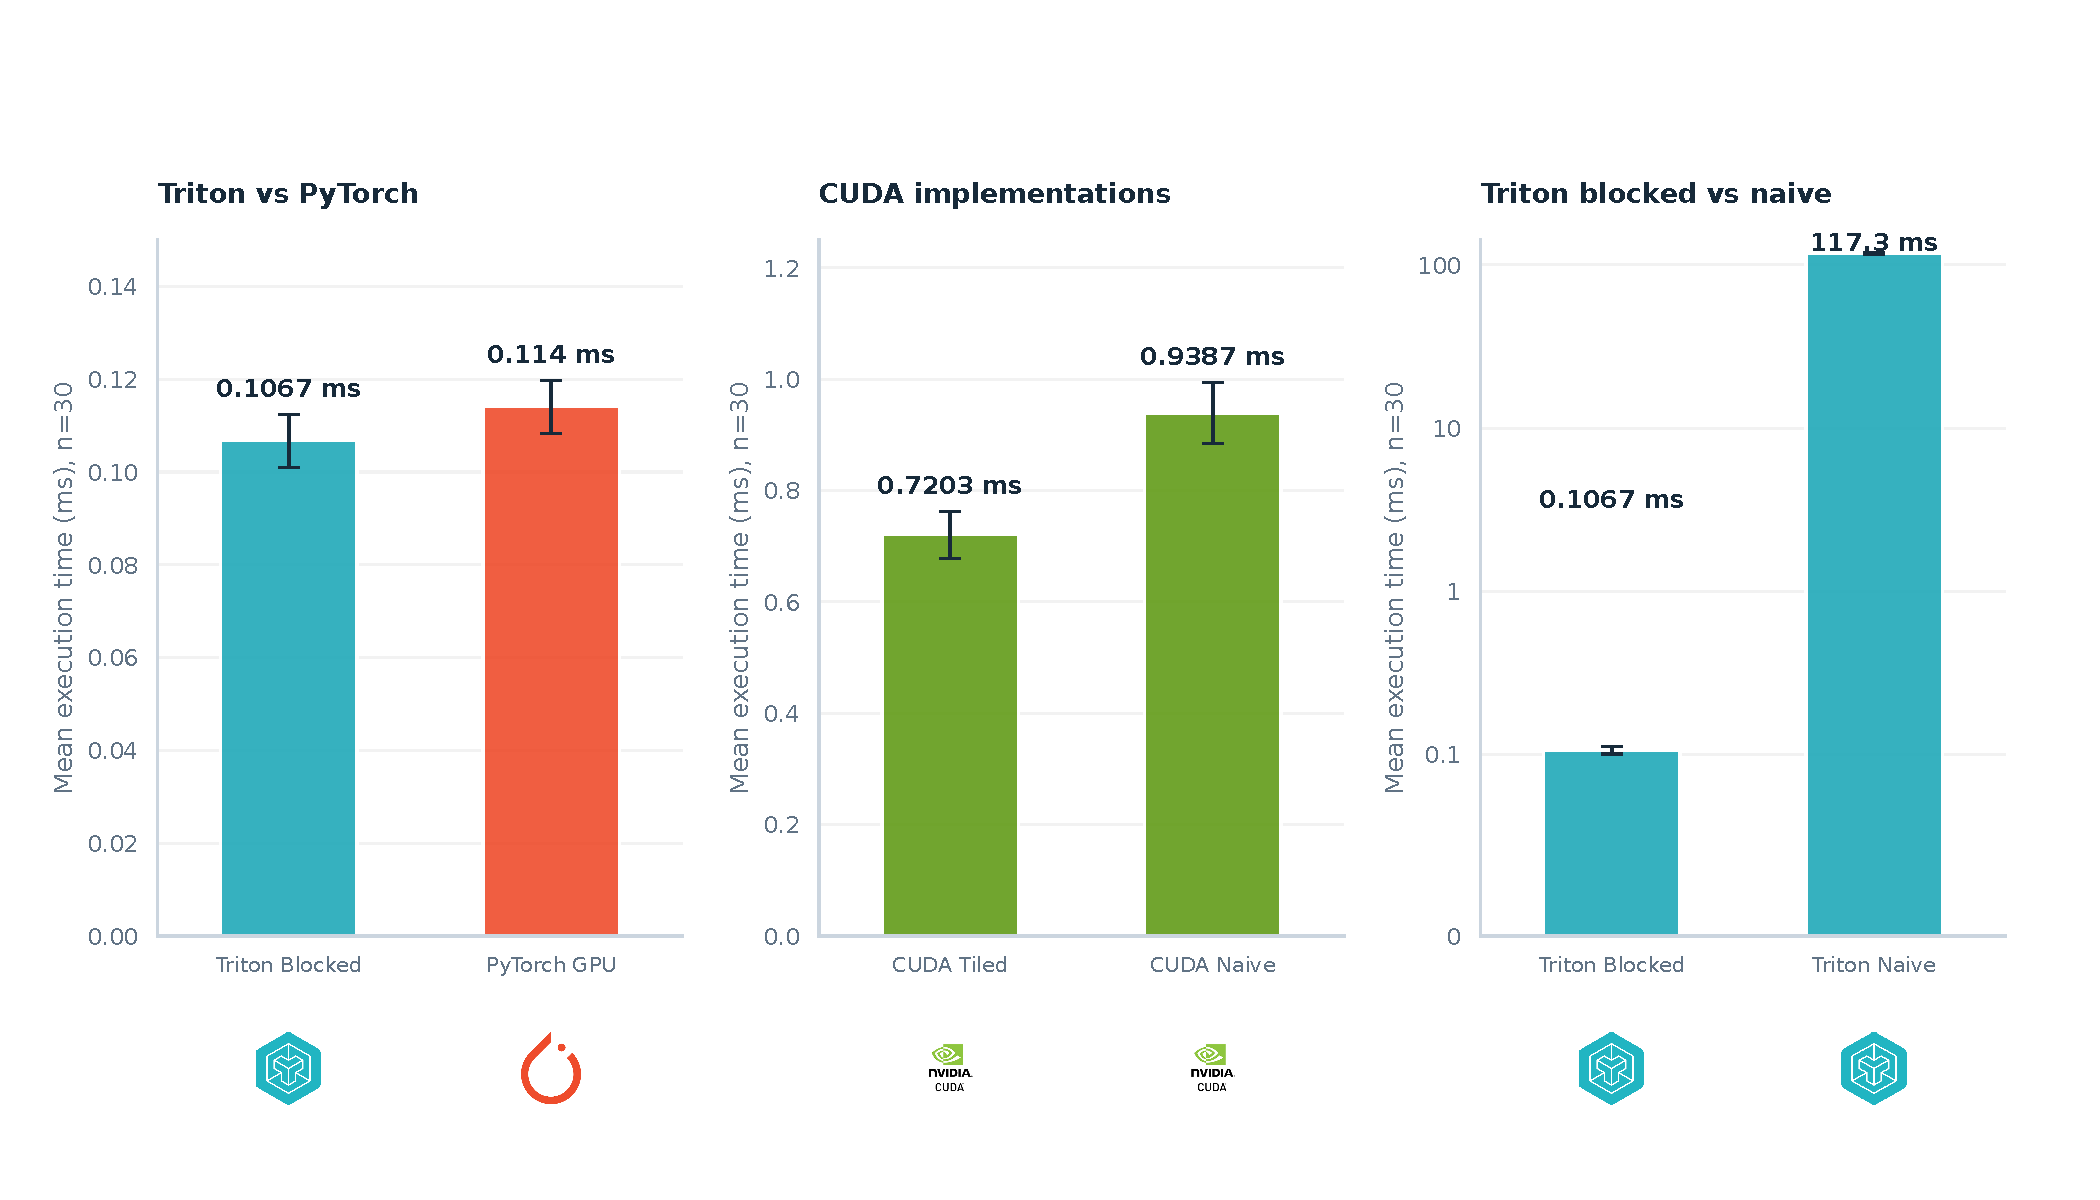
\includegraphics[width=0.98\textwidth,height=0.82\textheight,keepaspectratio]{02_gpu_detail.pdf}
  \caption{GPU execution time comparisons. The Triton blocked-versus-naive panel uses a symmetric logarithmic vertical scale to show both timings.}
  \label{fig:gpu-detail}
\end{figure}
\clearpage

\begin{figure}[p]
  \centering
  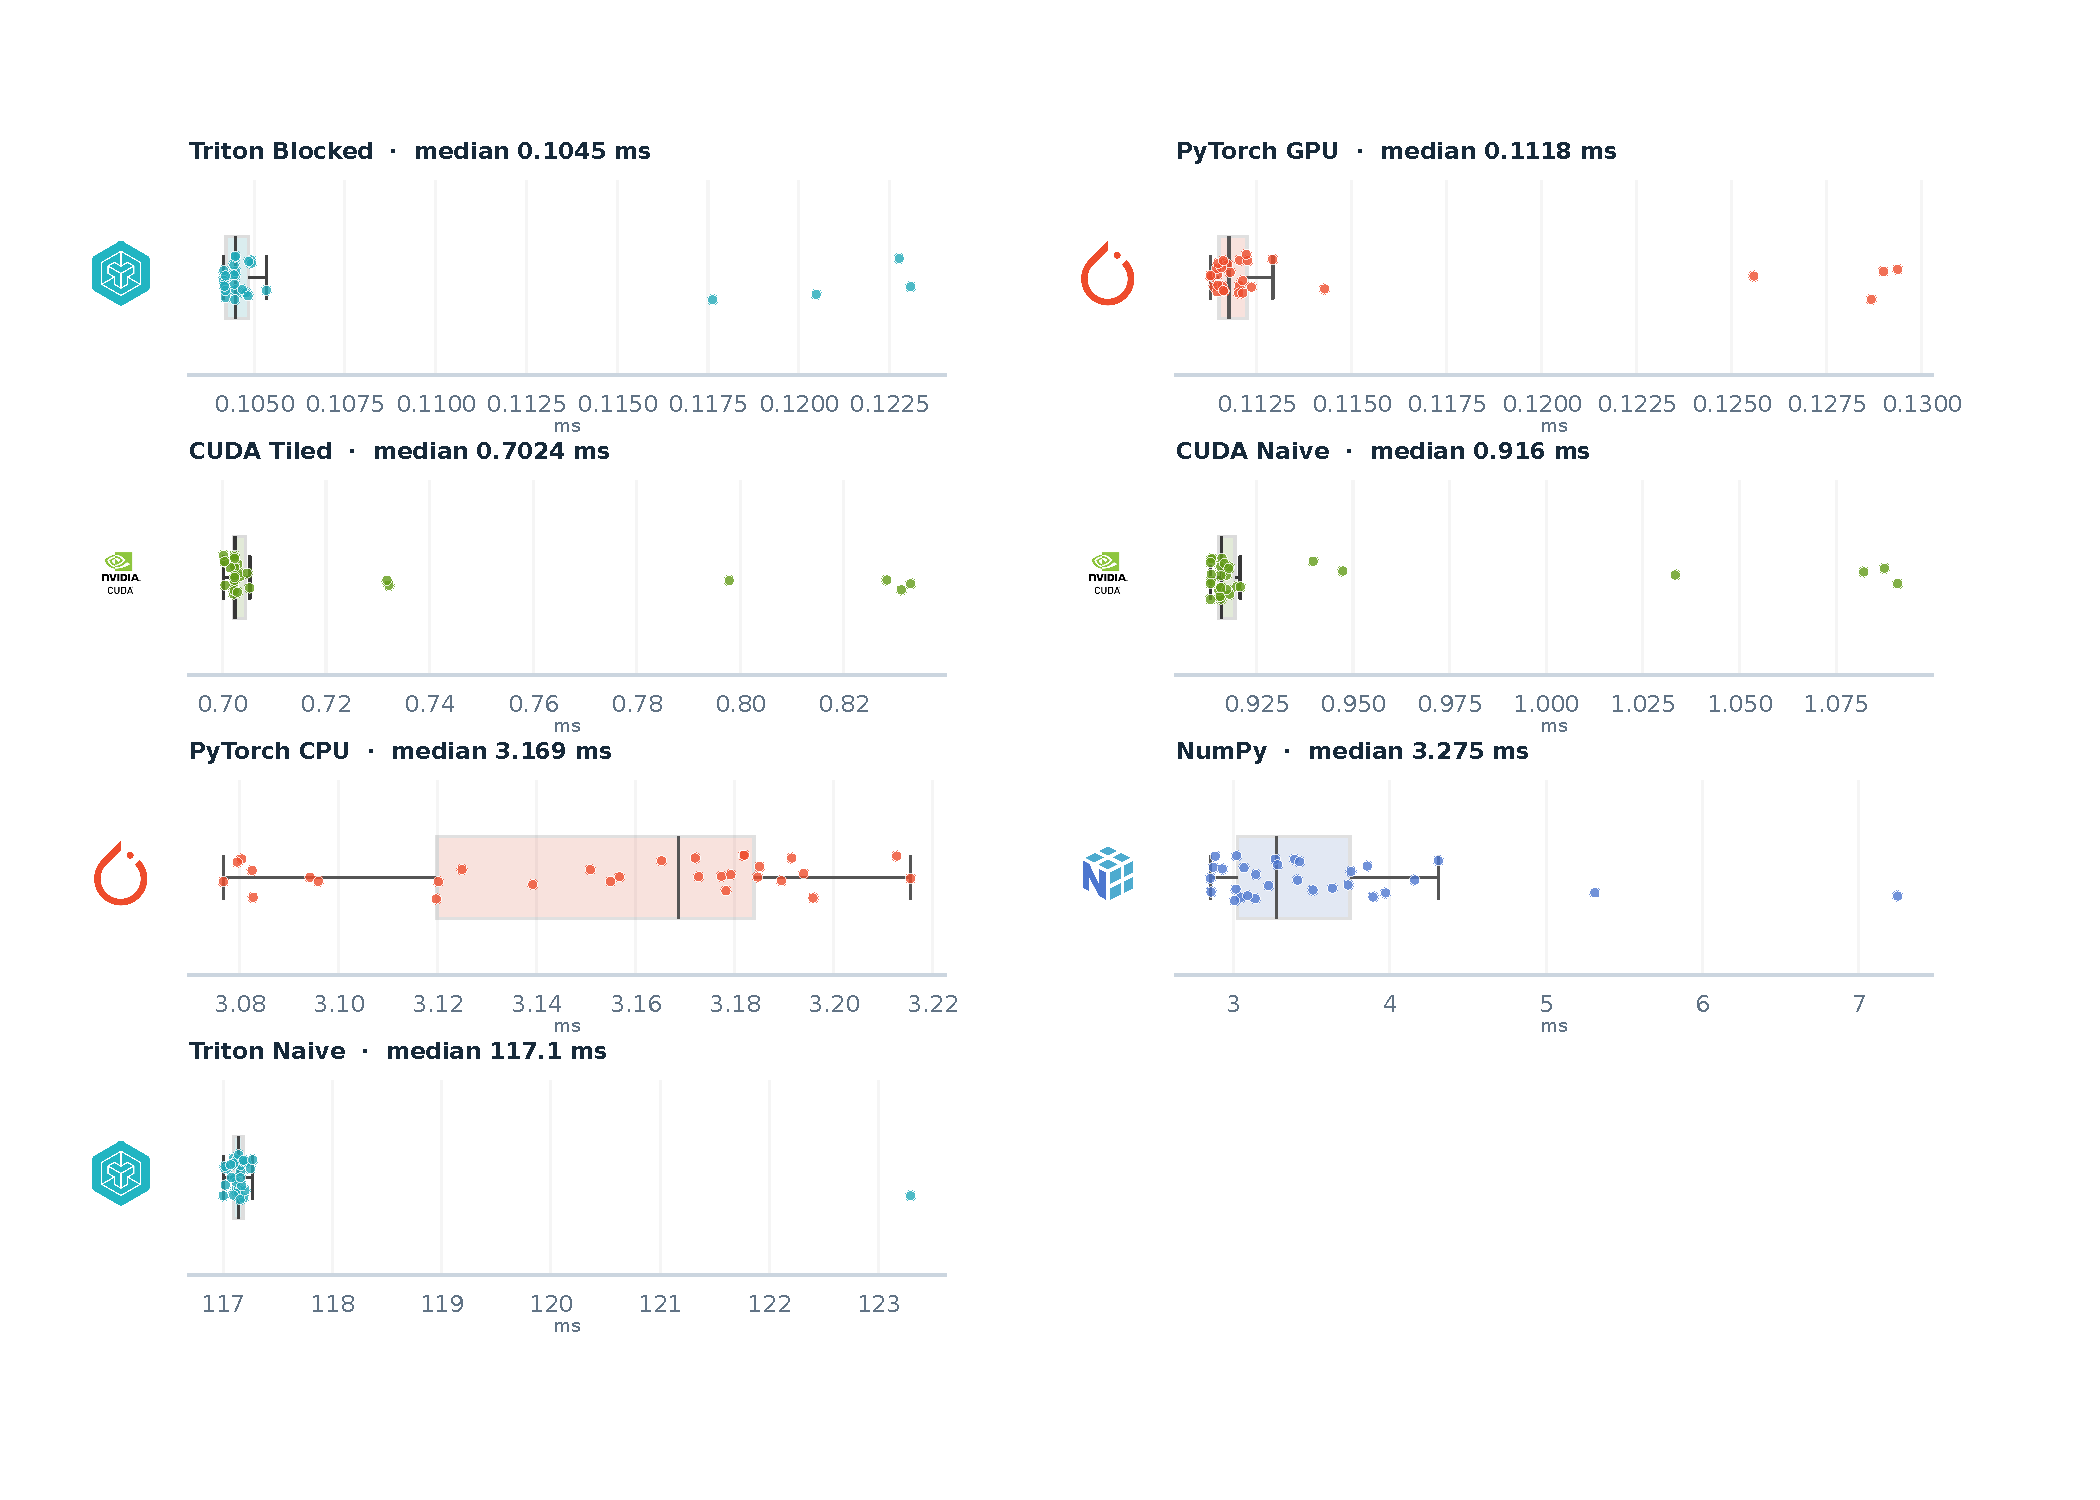
\includegraphics[width=0.98\textwidth,height=0.82\textheight,keepaspectratio]{03_distributions.pdf}
  \caption{Individual measured timing samples and their distributions. Each panel uses its own horizontal scale.}
  \label{fig:distributions}
\end{figure}
\clearpage

\begin{figure}[p]
  \centering
  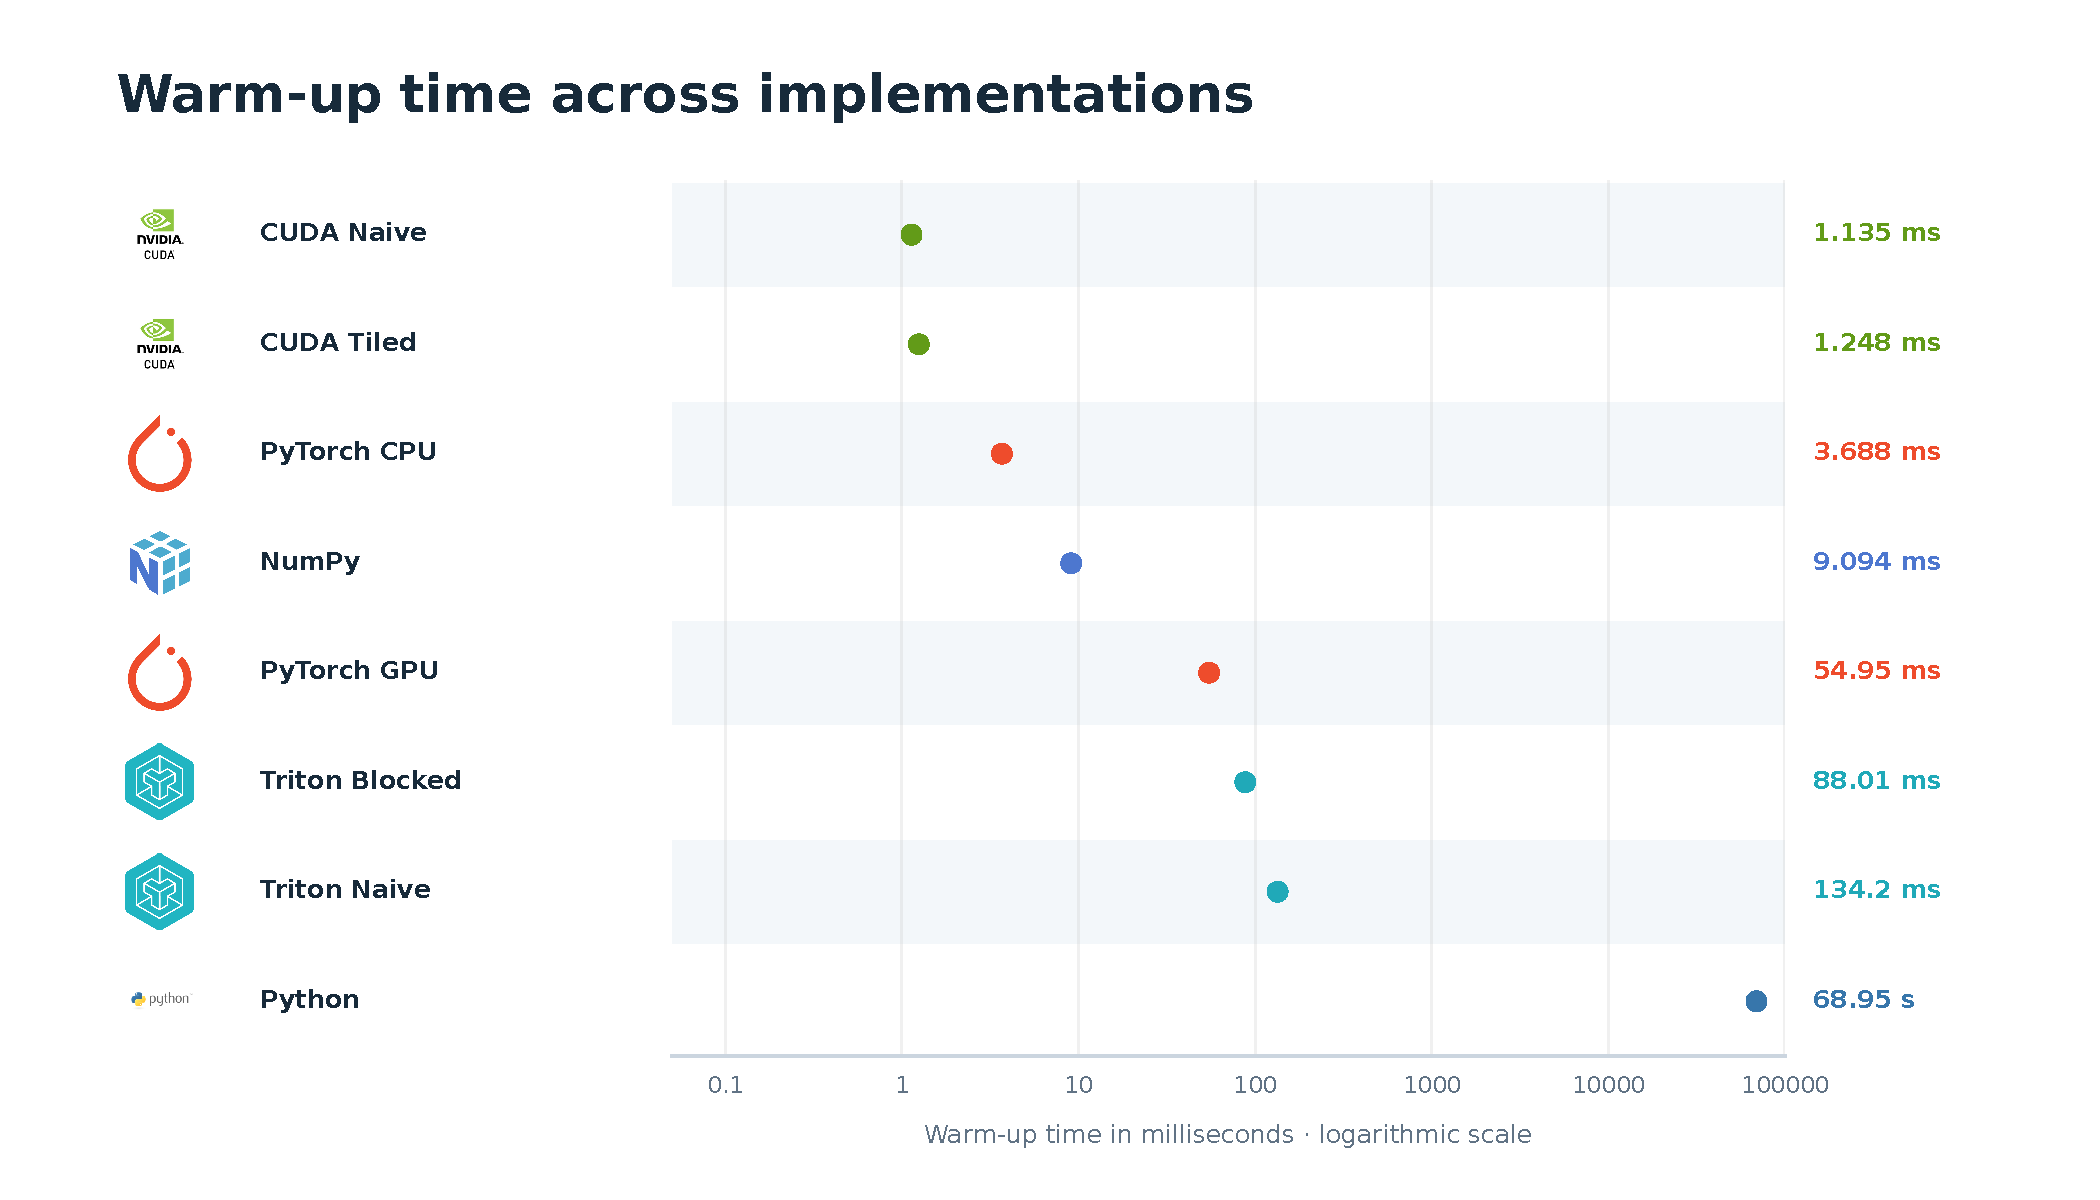
\includegraphics[width=0.98\textwidth,height=0.82\textheight,keepaspectratio]{04_warmups.pdf}
  \caption{Separately recorded warm-up times. These are not included in the execution-time sample statistics.}
  \label{fig:warmups}
\end{figure}
\clearpage

\begin{figure}[p]
  \centering
  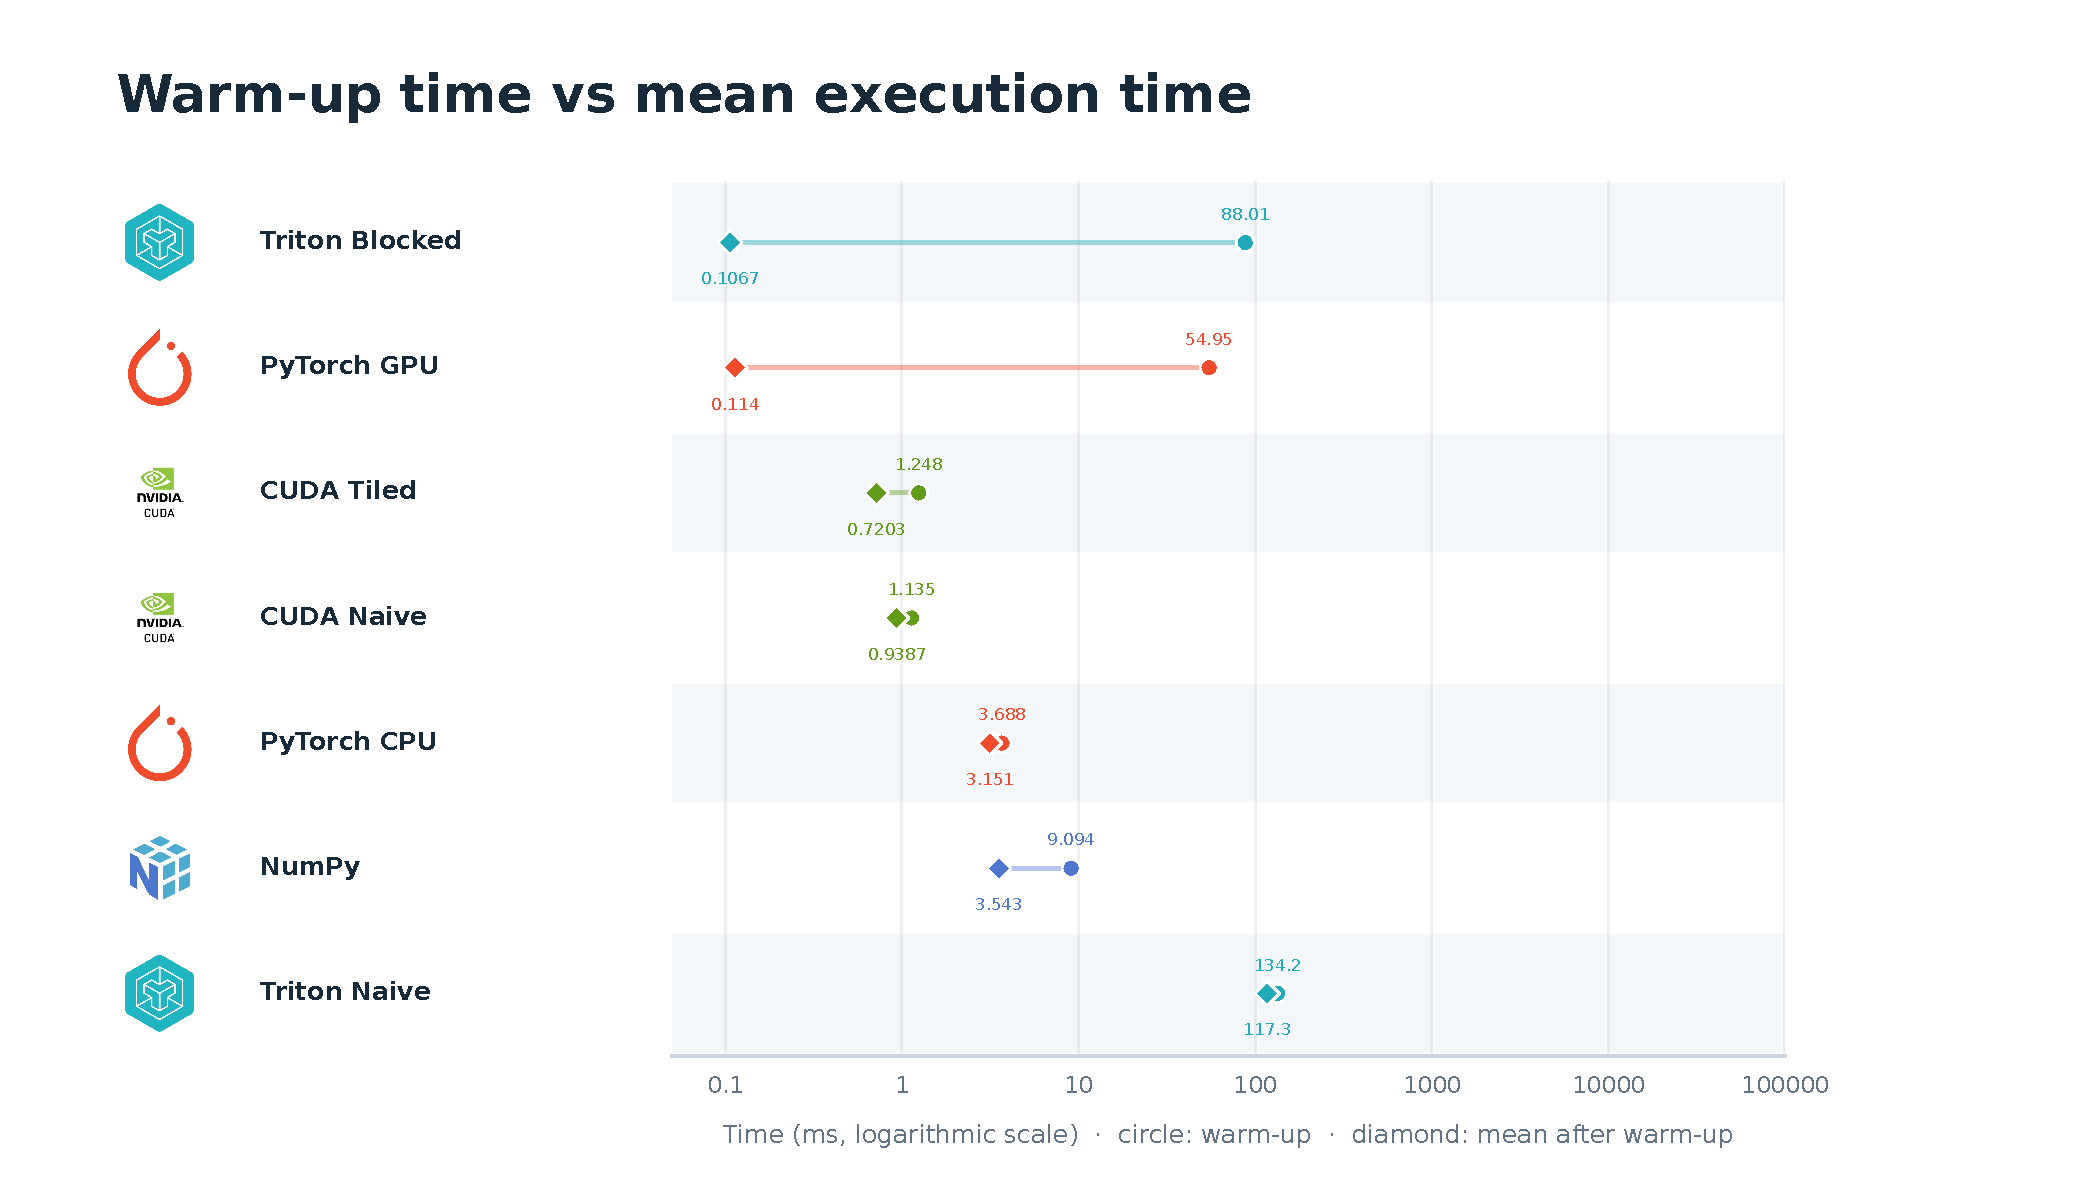
\includegraphics[width=0.98\textwidth,height=0.82\textheight,keepaspectratio]{05_warmup_vs_mean.pdf}
  \caption{Warm-up time and mean measured execution time for implementations with repeated samples. Circles show warm-ups; diamonds show measured means.}
  \label{fig:warmup-vs-mean}
\end{figure}
\clearpage

\section{Discussion}
% TODO: Interpret the naive-versus-blocked Triton results in terms of work per
% program, parallelism, data reuse, and arithmetic hardware. Discuss what the
% measurements support and what they cannot isolate (for example, tiling versus
% precision or library implementation).

\section{Limitations}
% TODO: Discuss correctness coverage, single-size/single-device scope, different
% CPU/GPU timing methods, precision differences, warm-up semantics, and the
% single pure-Python sample. Add any other limitations specific to your run.

\section{Conclusion}
% TODO: Answer the research question in a few sentences and identify one
% specific improvement or follow-up experiment.

\section*{Reproducibility}
% TODO: Give the command used to run the benchmark and identify the commit or
% archived source version. Results are written under ../Data/.

\begin{thebibliography}{9}
\bibitem{triton}
OpenAI, \emph{Triton documentation},
\url{https://triton-lang.org/main/}.

\bibitem{pytorch}
PyTorch contributors, \emph{PyTorch documentation},
\url{https://pytorch.org/docs/stable/}.

\bibitem{cuda}
NVIDIA, \emph{CUDA C++ Programming Guide},
\url{https://docs.nvidia.com/cuda/cuda-c-programming-guide/}.
\end{thebibliography}

\end{document}
